\chapter{本研究における課題定義と仮説}
\label{issue}

本章では,~\ref{background}章で述べた背景より,本研究における課題とその要件について議論し,
先行研究および提案システムを概説することで本研究で用いるアプローチについて述べる.

\section{本研究における課題定義}
\label{issue:definition}

本研究では、惑星規模の分散システムのテストのためのステージング環境の構築が困難であり、未だ整っていないことを課題とする。
~\ref{background}で述べた背景より、順を追って説明する。

モノリスや分散システムにおいて、開発者はサーバの配置や数を任意で決定することができる。
そのため、本番での実運用をする場合にオンプレ環境を用いる場合はステージング環境もオンプレ環境に、
クラウド環境を活用する場合はAWS~\cite{AWS}やGCP~\cite{GCP},Azure~\cite{Azure}といったクラウドサービスを利用することで,比較的簡単にステージング環境の構築を行える.
最近では,AWSのEKSやGCPのGKE, AzureのAKSなどクラウドサービス上でフルマネージドなKubernetesクラスタをクリックひとつで用意することが可能となっている.

対して、冒頭で述べたように惑星規模の分散システムにおいてはステージング環境の構築が困難である。
惑星規模の分散システムとは、分散システムの中でも地理的に分散配置されたコンピュータが協調動作することによってシステム全体が動作するものである。
さらに、開発者はシステムに参加するコンピュータの配置を固定化することはできず、システム全体もスケーリングする可能性がある。
よって、惑星規模の分散システムのステージング環境においては、実際に地理的な場所を指定し分散配置させたサーバが必要となる。
サーバを分散配置させた場合、システム全体を統合管理することが困難になる。
すべてのサーバに対し一斉にオペレーションを送ることが出来ないため、各地点のオペレータがアプリのインストールやアップデートといった作業を手作業で行う必要がある。
オペレータ同士での作業の確認や手作業を考慮すると、ステージング環境でのテストの開始までに多くの時間が掛かり、何らかの修正を加える度にこれらの作業を繰り返さなければならない。

そこで本研究ではOpenVPNとKubernetesを活用し,地理的かつネットワークにおいて論理的に離れたサーバをオーケストレーションすることにより惑星規模の分散システムのためのステージング環境を提案した.

\section{課題解決における要件}
\label{issue:requirements}

本節では、課題解決における要件を定義する。

惑星規模の分散システムをテストするためのステージング環境の構築には、サーバの配置に地理的な場所を指定し分散させる必要がある。
さらに、テストを円滑に進めるため、物理的に離れた場所に置かれたサーバに対して統括的な指示を出せることが求められる。
そこで、本研究の課題解決のための要件として、実際性・統合性・拡張性の三つを挙げた。

\subsection{実際性}
\label{issue:requirements1}

P2Pシステムの検証は,実際のネットワーク上で行う必要がある.
テスト等の論理的検証では不十分である.
P2Pシステムでは,状況に応じてノード同士の関係性・役割が変化し,条件が固定的でないからである.
複雑な条件下での運用が必要であるから,ステージング環境においても,実際に地理的に分散したノードによるネットワークが求められる.

\subsection{統合性}
\label{issue:requirements2}

ステージング環境においては,ある地点から全てのノードを統合的に操作できる必要がある.
現状,アプリケーションの配布・実行・停止等において多大なコミュニケーションコストとヒューマンリソースのオーバーヘッドが課題となっており,
システム内のノードの管理に統合性を持たせることによってこれらのオーバーヘッドを削減する必要がある.

\subsection{拡張性}
\label{issue:requirements3}

ステージング環境では,アプリケーションの修正に伴うアップデートならびにノード数の増加・減少といった変化への柔軟性が必要である.
P2Pシステムは刻一刻と変化するシステムであること.ノードの数によって関係性が変化する.
また,ステージング環境では頻繁なアップデートが予想され,その際に生じるオーバーヘッドの削減が必要である.

\section{先行研究}
\label{issue:previous-research}

P2Pシステムのためのステージング環境の構築手法としては,すでにいくつかの先行研究が存在する.

\subsection{独自実装のデバッグエージェントによるテスト}

既存の提案として,地理的に分散したノードを統合管理・操作するために別アプリケーションを独自で開発する手法がある.
別アプリケーションとは,対象アプリケーションに対して命令を送信したり通信内容をログとして抽出するなどのデバッグエージェントして動作する.
ノードを統合管理出来る点では要件を満たしており,コミュニケーションならびに工数の削減に繋がると考えられる.
しかし対象アプリケーションにパッチを適用したい場合,同様にそれを操作するデバッグエージェントにも変更を加える必要があり,変更への弱さが窺える.
アップデートへの柔軟性が不足している限り,それによって生じるオーバーヘッドを削減することが出来ず根本的な解決に繋がらないと思われる.
分散したノードを一斉にコントロールだけでなく,アプリケーションの停止や更新といった変更においてもより少ない手間で抑えられることが求められ,
それを満たした際に惑星規模の分散システムの十分なステージング環境が成り立つと考えられる.

\subsection{PlanetLab}
\label{consideration:related-works:planetlab}

惑星規模のサービスを開発するためのオープンなプラットフォームとして,PlanetLab~\cite{PlanetLab}が挙げられる.
PlanetLabは,新規サービスの開発をサポートするグローバルな研究ネットワークであり,900以上のノードから構成される.
2003年から始動し,1000人以上の研究者が分散ストレージ,ネットワークマッピング,P2Pシステム,分散ハッシュテーブルなどの
新たな技術の開発のためにPlanetLabを利用している.
それぞれのノードは仮想マシンを提供しており,ユーザに割り当てられた仮想マシンのセットはSliceと呼ばれている.
ユーザはsocket APIを通じて個別の開発環境を構築することが可能であり,sshを通して仮想マシンにアクセスしアプリケーションを
デプロイできる.

\subsection{Emulab}
\label{consideration:related-works:emulab}

分散システムや分散ネットワークを,ネットワークエミュレータによって構築された仮想的なネットワーク上で研究や開発する取り組みとしては,
Emulab~\cite{Emulab}が挙げられる.
Emulabは大規模なソフトウェアシステムであり,仮想ネットワーク内に点在するマシン同士の接続環境を自由に設定することが可能である.
ネットワークエミュレータを活用し,開発環境で大規模な分散システムのための開発環境を構築する手法
~\cite{RelatedWork1}も提案されている.
数台のコンピュター上に数千台の仮想環境をプロセスレベルで構築し,それらをネットワークシミュレータにより相互接続することによって,
擬似的なネットワーク環境においての動作検証を可能にするものである.

\section{本研究における仮説}
\label{issue:hypothesis}

本研究では~\ref{issue:requirements}章で述べた実際性,統合性,拡張性を担保しながら地理的に分散したシステムのためのステージング環境を構築したい.
そこで,OpenVPNとKubernetesを活用することで,それらの要件を満たしたシステムが構築できるのではないだろうかと考えた.
それぞれの要件に対して,本研究で提案するシステムによる実現が可能であると考えられる点を本節では述べる.

\subsection{実際性}

OpenVPNを活用することで,ネットワーク上で論理的に異なるセグメントに位置するノード同士で疎通が可能なオーバーレイネットワークを構築することができる.
さらに,IP Reachableな条件下であればKubernetesによるクラスタリングが可能である.よって,実際のネットワーク上にステージング環境を構築することが
可能となり,P2Pシステムの検証における実際性が担保されると考えられる.

\subsection{統合性}

Kubernetes自体がオーケストレーションシステムであり,Kubernetesクラスタに参加するワーカーノードはマスターノードからの統合管理が可能である.
そのため本研究では,P2Pシステムに参加するノードをKubernetesクラスタのワーカーノードとして運用することで,マスターノードを経由したアプリケーション
の配布や実行が可能となり,統合性が担保されると考えられる.

\subsection{拡張性}

Kubernetesではアプリケーションをコンテナとして動かすため,ワーカーノード内でコンテナ数を増減したり,コンテナのアップデートを行える.
また,本研究ではKubernetesクラスタ構築時にkubeadmを使用しており,これを用いることで新たなノードをクラスタに参加させることも可能となる.
これによって,修正が重なる可能性のあるステージング環境に必要な拡張性が担保されると考えられる.

\section{提案システム概要}
\label{issue:about-system}

提案システムの概要を述べる.ステージング環境においてP2Pシステムに参加するノード同士を,OpenVPNを利用することで相互に疎通可能な状態にする.
OpenVPNオーバーレイネットワーク上でKubernetesクラスタを構築し,全てのノードをクラスタに参加させる.Kubernetesクラスタ内のマスターノードを
介して,全てのノードに対して操作を行うことができる.

\begin{figure}[htbp]
  \begin{center}
    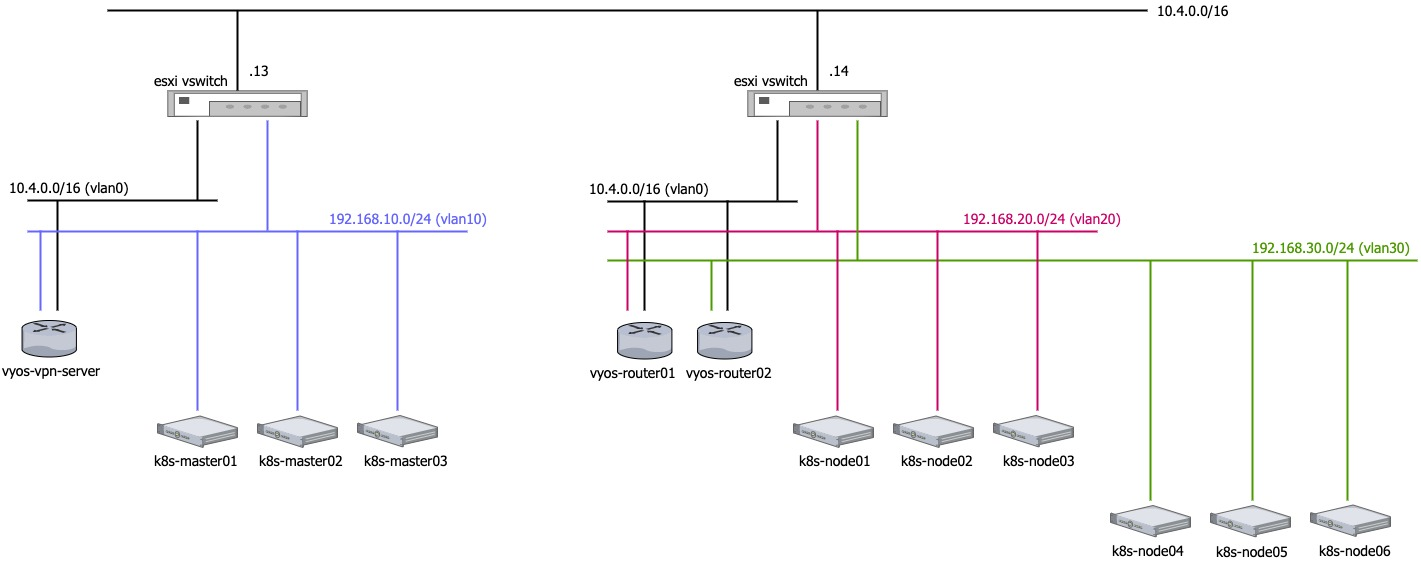
\includegraphics[width=\textwidth]{./figures/system-diagram.jpg}
    \caption{システム概要図}
  \end{center}
\end{figure}

%%% Local Variables:
%%% mode: japanese-latex
%%% TeX-master: "./thesis"
%%% End:
